\section{Конструкторская часть}

\subsection{Постановка задачи проектирования}

Подсистема работы с текстовыми данными на географической карте <<Вохв-ГЕО>> позволяет проводить накопление и анализ новостных документов с помощью формализованного языка запросов для отображения на карте. Данная подсистема предназначена для исследовательской деятельности и для включения в состав сложных комплексов анализа событий в новостных потоках.

Подсистема «Волхв-ГЕО» должна выполнять следующие функции
\begin{itemize}
\item Удаленный доступ к системе. Программное изделие должно обеспечивать удаленный доступ к системе через Web-сервер.
\item Соединение с базой данных. Программное изделие должно осуществлять удаленное соединение с базой данных.
\item Ввод с клавиатуры. Данные, вводимые с клавиатуры должны иметь тип и формат, соответствующий типу и формату полей записи.
\item Добавление информации в базу данных. Программное изделие должно осуществлять добавление новой записи в базу данных при условии, что эта запись удовлетворяет всем требованиям, налагаемым на входные данные.
\item Удаление информации из базы данных. Программное изделие должно осуществлять исключение выбранной пользователем записи в таблице из исходной базы данных.
\item Редактирование информации в базе данных. Функция должна осуществлять редактирование поля записи, выбранного пользователем. При этом при редактировании данных должны выполняться все требования, налагаемые на входные данные.
\item Геопривязка новостей.
\item Анализ динамики новостей.
\item Отображение данных на карте. Функция должна осуществлять отображение новостной информации на карте.
\item Создание сценариев. Функция должна обеспечивать создание и редактирование сценария – набора визуальных элементов на карте.
\item Создание аналитической заметки. Функция должна обеспечивать создание и редактирование аналитической заметки – текстового сопровождения к сценарию
\end{itemize}

%\clearpage
\subsection{Описание предметной области}
\subsubsection{Естественно-языковая модель предметной области}

На данный момент существует очень мало систем, позволяющих проводить работу с новостными данными на географических картах. Ближайшие аналоги предоставляют отображение на карте новостной информации, предоставленной пользователями, собранной и обработанной в ручном режиме.

Подсистема <<Волхв-ГЕО>> должна работать в составе более крупной АИС, обеспечивая отображение собранных новостных данных на карте и должна предоставлять инструментарий по прогнозированию ситуаций и построению аналитических заметок. Подсистема использует формализованные запросы для решения задачи геотегирования текстов: формализованный запрос может определять географические привязки новостных сообщений путем учета упоминаемых географических названий. К результатам такого запроса можно привязать географические метки, чтобы использовать их в более сложных запросах.

Для реализации этой задачи требуется база новостей и система полнотекстового поиска по индексированным документам, которая не входит в структуру проектируемой подсистемы и является внешней системой, обозначаемой ИПС.

Требования, накладываемые на ИПС:
\begin{itemize}
\item Поддержка полнотекстового индекса
\item Поддержка полнотекстовых запросов
\item Поддержка запросов с учётом морфологии языка
\item Поддержка сохранённых запросов
\item Возможность редактирования документов посредством API
\item Поддержка текстовых меток
\end{itemize}

Подсистема Волхв-ГЕО, используя сохранённые в своей базе запросы, опрашивает ИПС. Полученные документы помечаются соответствующей геометкой. Используя запросы, сохранённые в ИПС, подсистема Волхв-ГЕО получает документы по требуемым темам и сохраняет агрегированные значения в собственной базе для последующего анализа.
По агрегированным значениям из собственной базы подсистема проводит анализ и результаты анализа сохраняются для дальнейшего использования аналитиком.

Первичной задачей является разметка документов геометками. За исключением случаев, когда координаты места события предоставлены в тексте новости, невозможно в автоматическом режиме точно привязать событие к конкретной точке земной поверхности.

Поэтому представляется нецелесообразным использование в качестве меток географических координат -- широты и долготы. В процессе проектирования было принято решение в качестве минимального географического объекта принять субъекты первого уровня, в рамках подсистемы называемые <<провинциями>>. Например, для Российской Федерации это соответствует субъекту федерации, для США -- штату, для Армении -- марзу.

Согласно стандарту ISO 3166, каждому государству соответствует двух и трёхбуквенный код, а каждому субъекту первого уровня -- код, состоящий из кода страны и кода субъекта.
Код страны/субъекта является текстовой меткой, используемой в подсистеме.

Для провинций, присутствующих в стандарте используется код из стандарта. Для провинций не присутствующих в стандарте, в основном это непризнанные территории, вводится собственное кодовое обозначение по методике, принятой в стандарте.

Результатом работы пользователя в подсистеме является сценарий развития ситуации, и аналитическая записка.

Сценарий представляет из себя набор графических элементов карты с сопроводительным текстом.

Аналитическая записка включает в себя текстовое описание текущей ситуации, сценария развития ситуации и иную информацию по необходимости.

Предметная область разработанной автоматизированной системы представлена на
рисунке~\ref{figure:domain}.

\begin{figure}[!h]
\centering
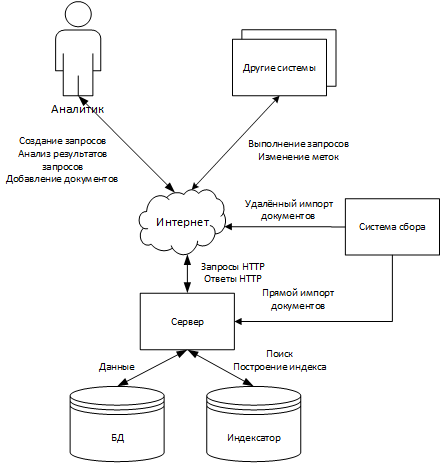
\includegraphics{design/domain}
\caption{Схема предметной области.}
\label{figure:domain}
\end{figure}

\clearpage
\subsubsection{Сущности предметной области}

В процессе анализа предметной области выделены основные сущности:
\begin{itemize}
\item Запрос;
\item Прогноз;
\item Регион;
\item Страна;
\item Провинция;
\item Сценарий;
\item Аналитическая записка;
\end{itemize}

Дополнительные сущности, наличие которых следует из основных:
\begin{itemize}
\item Полином -- параметры полинома в полиноминальной регрессии
\item Скользящее среднее -- параметры для алгоритма скользящего среднего
\item Измерение прогноза -- сохранённый результат выполнения запроса прогноза по дням;
\item Популяция прогноза -- коллекция формул для прогноза;
\item Приспособленность -- история лучших и средних значений функции приспособленности по поколениям для популяции;
\item Веса -- веса для итоговой оценки методом средневзвешенной суммы
\end{itemize}

Выявлены следующие акторы:
\begin{itemize}
\item Пользователь -- основной пользователь подсистемы
\item Эксперт -- создаёт/редактирует запросы, редактирует контура стран/провинций
\end{itemize}

Выявлены следующие источники данных:
\begin{itemize}
\item ИПС -- предоставляет API доступа и редактирования к актуальной базе новостей
\item Эксперт -- создаёт/редактирует запросы, редактирует контура стран/провинций
\end{itemize}

\subsubsection{Описание бизнес-процесса}
Автоматизации подлежат следующие процессы системы:
\begin{itemize}
\item Разметка документов базы геометками;
\item Прогнозирование новостных потоков;
\item Построение сценария развития ситуации;
\item Создание аналитической записки;
\end{itemize}

Новости агрегируются в ИПС. Модуль геотегирования размечает новости согласно сохранённым в Волхв-ГЕО запросам. Размеченные новости используются для прогнозирования ситуации и отображения на карте.

Схема бизнес-процесса представлена в графической части на листе <<Бизнес-процесс подсистемы>>

\begin{figure}[!h]
\centering
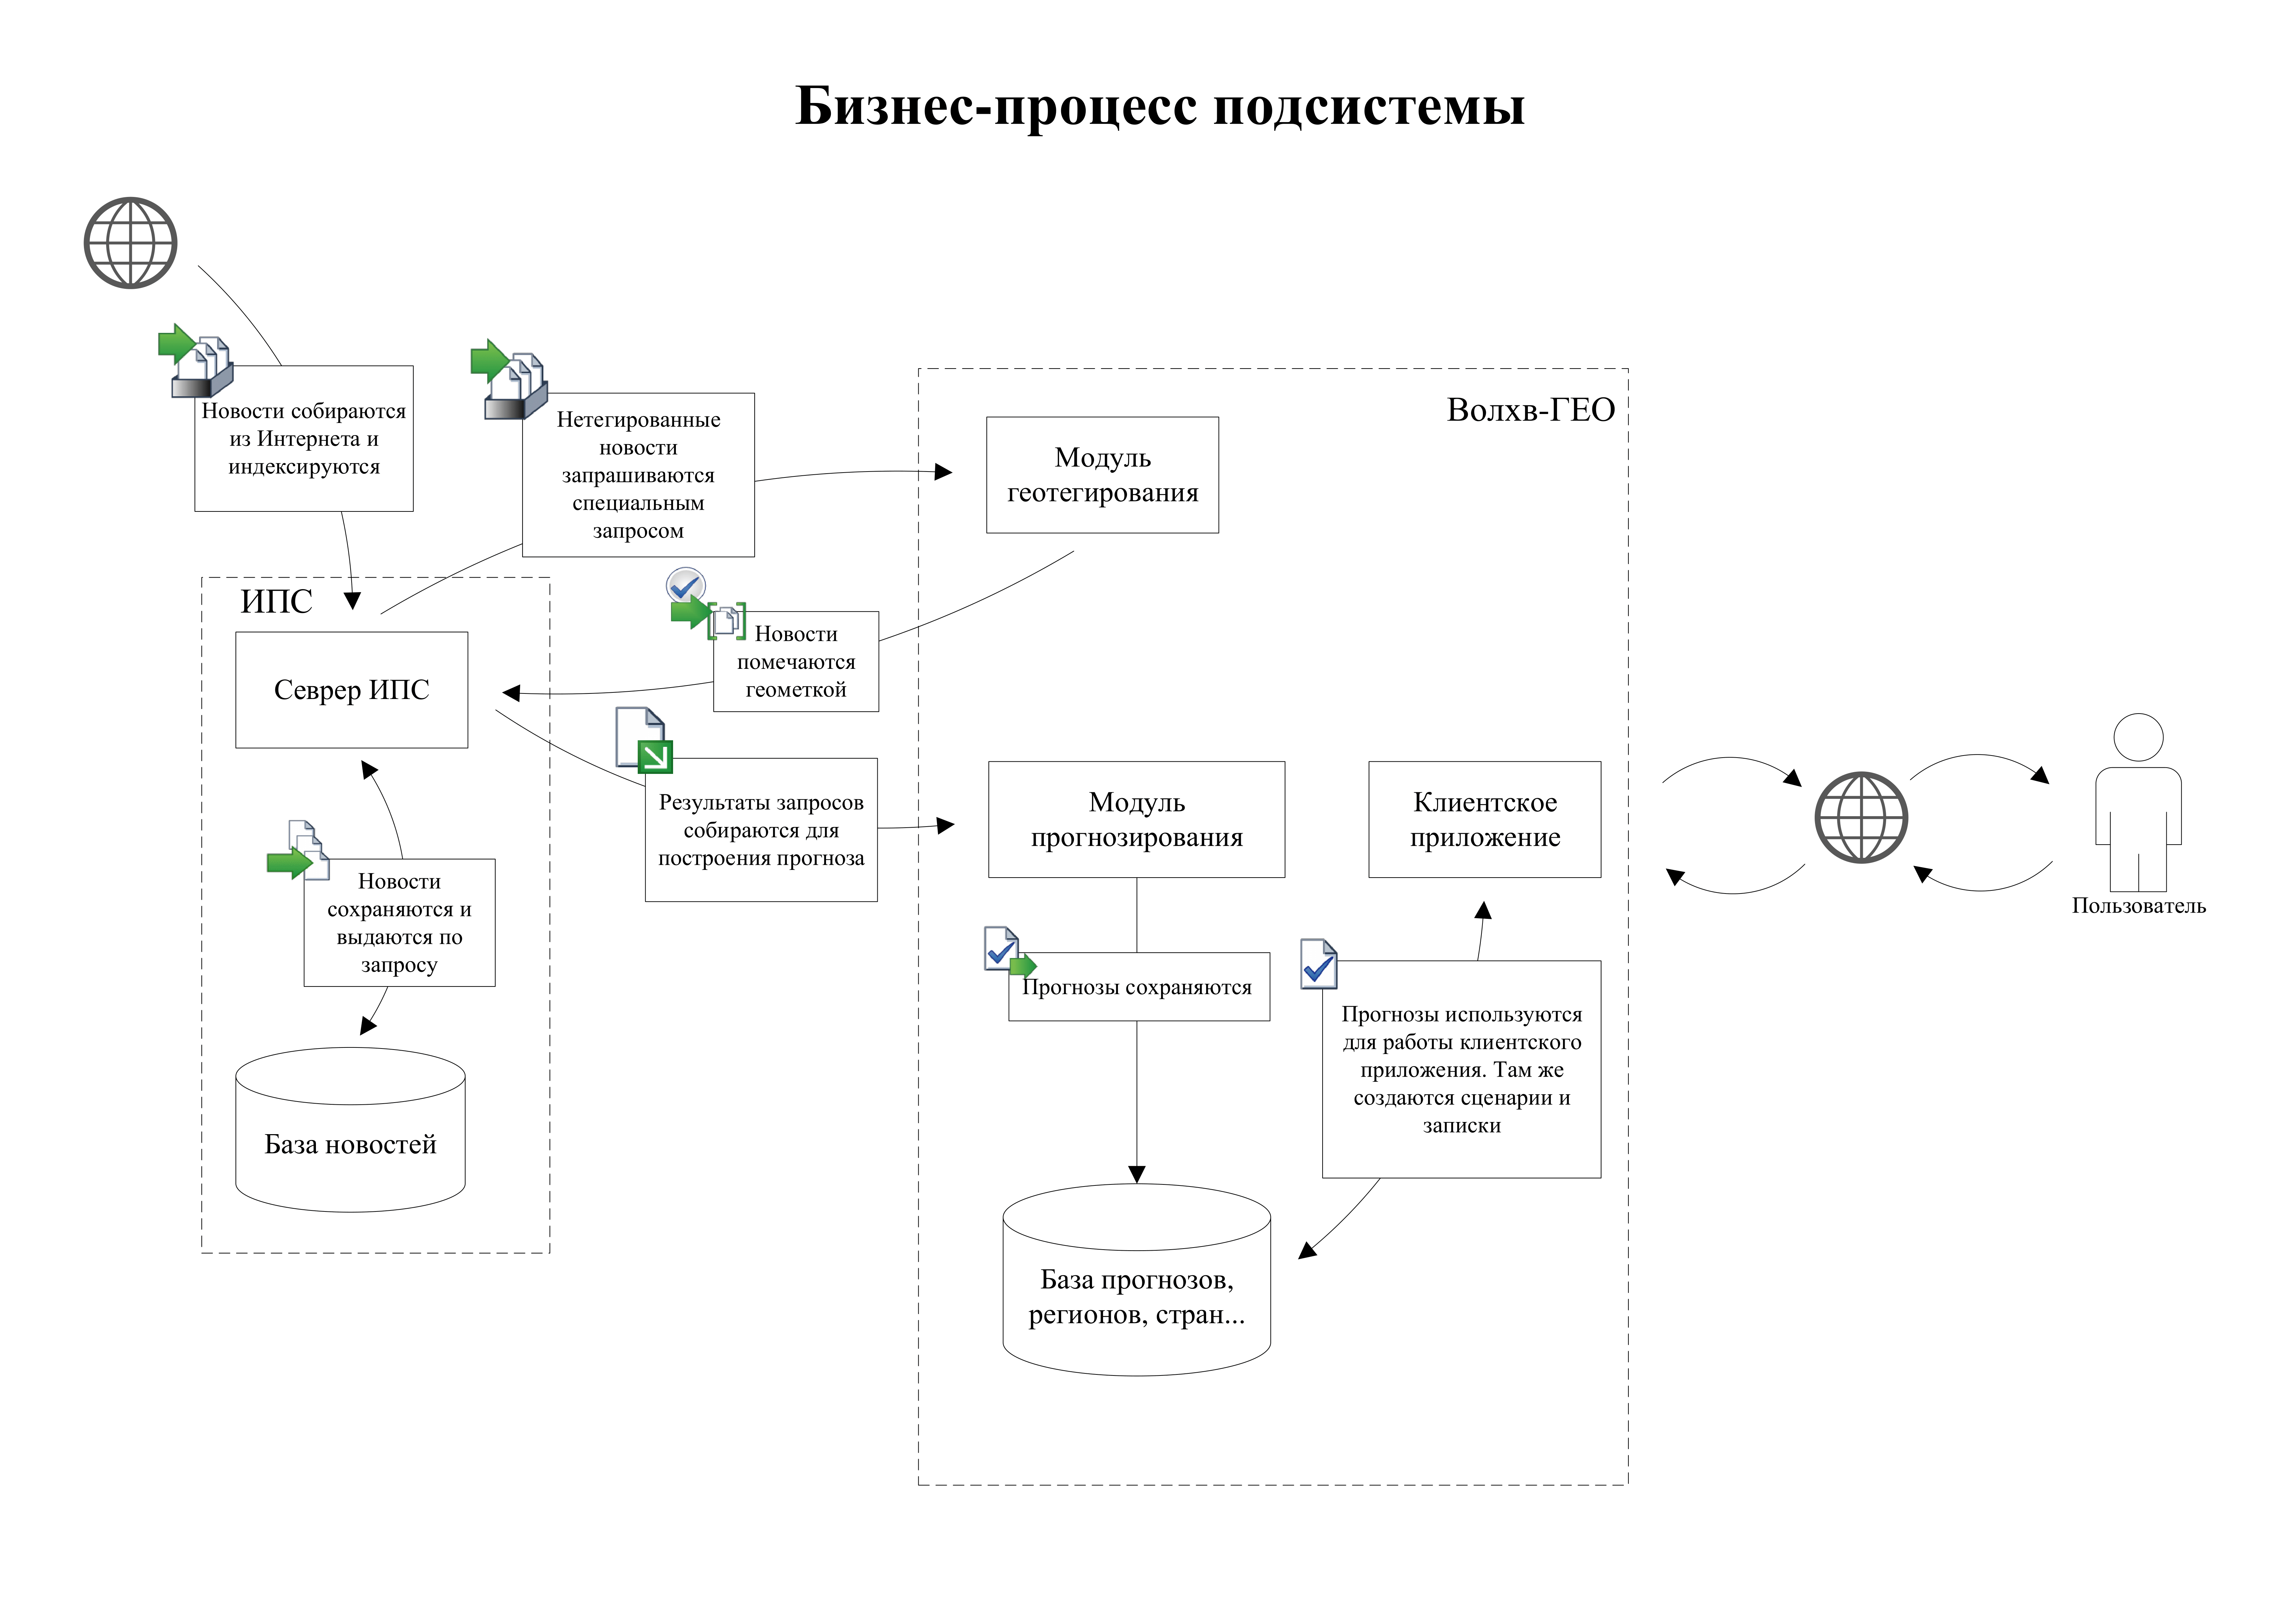
\includegraphics[width=\textwidth]{design/ramkaless/5.png}
\label{figure:businessProc}
\caption{Бизнес-процесс подсистемы.}
\end{figure}

\subsubsection{Выбор и обоснование критериев качества}

Для данной подсистемы можно выделить следующие критерии качества:
\begin{itemize}
\item Пользовательский интерфейс;
\item Геопривязка;
\item Автоматизация;
\item Интеграция;
\item Прогноз;
\item Сценарии.
\end{itemize}

\paragraph{Пользовательский интерфейс.}
Означает простоту и понятность работы с системой. Оценивается:
\begin{itemize}
\item Структура сайта;
\item Степень интуитивной понятности меню;
\end{itemize}

\paragraph{Геопривязка.}
Означает точность привязки события на карте. Оценивается:
\begin{itemize}
\item Информативность геопривязки;
\item Отклонение геометки от реального места событий.
\end{itemize}

\paragraph{Автоматизация.}
Оценивает количество функций выполняемых в автоматическом режиме.

\clearpage
\paragraph{Интеграция.} 
Обозначает возможность и удобство интеграции подсистемы с другими системами. Оценивается:
\begin{itemize}
\item Наличие интеграционного интерфейса;
\item Удобность этого интерфейса для разработчиков;
\item Полнота интерфейса (полная реализация всех возможностей системы в интерфейсе).
\end{itemize}

\paragraph{Прогноз.} 
Обозначает наличие прогнозирующего функционала и качество прогноза. Оценивается:
\begin{itemize}
\item Возможность автоматизированного прогнозирования;
\item Качество прогноза;
\end{itemize}

\paragraph{Сценарии.} 
Обозначает наличие инструментария для создания и редактирования сценариев и аналитических заметок. Оценивается:
\begin{itemize}
\item Наличие инструментария;
\item Качество инструментов;
\end{itemize}

Присвоим критериям качества следующие весовые коэффициент, которые отображены в таблице~\ref{table:qualityWeights}.

\begin{table}[h!]
\centering
\caption{Критерии качества и их весовые коэффициенты}
\label{table:qualityWeights}
\begin{tabular}{L{10cm}|C{3cm}}
\multicolumn{1}{C{10cm}|}{Критерий} & 
\multicolumn{1}{C{3cm}}{$\alpha$} \\
\hline\hline

Пользовательский интерфейс & 0.1 \\
Геопривязка & 0.2 \\
Автоматизация & 0.25 \\
Интеграция & 0.15 \\
Прогноз & 0.2 \\
Сценарии & 0.1 \\

\end{tabular}
\end{table}

Выполнено следующее условие:
\begin{equation}
\sum \alpha_i = 0.1 + 0.2 + 0.25 + 0.15 + 0.2 + 0.1 = 1
\end{equation}

\subsubsection{Перечень задач, подлежащих решению в процессе разработки}

В процессе разработки необходимо решить следующие задачи:
\begin{itemize}
\item исследование и анализ предметной области;
\item анализ и определение критериев качества;
\item определение функциональных требований разрабатываемой системы;
\item разработка структуры модулей системы, с выделением функциональности для каждого модуля;
\item проектирование базы данных: инфологическая, даталогическая модели;
\item проектирование эволюционного алгоритма прогнозирования;
\item рассмотрение и обоснование архитектуры системы;
\item выбор программных библиотек для реализации модулей;
\item разработка интерфейса взаимодействия пользователя с программой;
\item реализация графа диалога;
\item написание и отладка программного кода модулей системы;
\item разработка технической документации.
\end{itemize}

\clearpage
\subsubsection{Анализ аналогов и прототипов}

Для расчета нормированного значения j-го варианта по i-ому критерию необходимо
воспользоваться формулой~\ref{equation:criteria}.

\begin{equation}
\label{equation:criteria}
K_{ij} = \frac{x_{ij} - x_i^-}{x_i^+ - x_i^-}
\end{equation}
\begin{ESKDexplanation}
\item[где ] $x_{ij}$ - натуральное значение;
\item       $x_i^+$ - максимальное значение;
\item       $x_i^-$ - минимальное значение.
\end{ESKDexplanation}

Для расчета интегрального показателя воспользуемся формулой~\ref{equation:criteriaTotal}.

\begin{equation}
\label{equation:criteriaTotal}
K = \sum_{i=1}^m \alpha_i K_{ij}
\end{equation}
\begin{ESKDexplanation}
\item[где ] $m$ - количество критериев.
\end{ESKDexplanation}

Оценка по критериям производится путём присуждения баллов в соответствии со шкалой, представленной в таблице~\ref{table:criteria}.

\begin{table}[h!]
\centering
\caption{Критерии качества и их весовые коэффициенты}
\label{table:criteria}
\begin{tabular}{L{4cm}|C{2cm}|C{2cm}|C{2cm}|C{2cm}|C{2cm}}
\multicolumn{1}{C{4cm}|}{Качественный показатель} & 
\multicolumn{1}{C{2cm}|}{Отлично} & 
\multicolumn{1}{C{2cm}|}{Хорошо} & 
\multicolumn{1}{C{2cm}|}{Удовлетворительно} & 
\multicolumn{1}{C{2cm}|}{Плохо} & 
\multicolumn{1}{C{2cm} }{Неудовлетворительно} \\
\hline\hline

Количественный показатель & 5 & 4 & 3 & 2 & 1 \\
$K_{ij}$ & 1 & 0.75 & 0.5 & 0.25 & 0 \\

\end{tabular}
\end{table}

Прямых и полных аналогов проектируемой подсистемы нет, но есть проекты, реализующие части функционала:
\begin{itemize}
\item http://liveuamap.com/
\item http://militarymaps.info/
\end{itemize}

\clearpage
Эти аналоги имеют ряд принципиальных недостатков и не могут отвечать всем
требованиям.

Недостатками аналога «http://liveuamap.com/» являются:
\begin{itemize}
\item отсутствие системы прогнозирования;
\item отсутствие инструментария для создания сценария и аналитических записок;
\item узкий набор отслеживаемых тем;
\item невозможность добавить новость.
\end{itemize}

Недостатками аналога «http://militarymaps.info/» являются:
\begin{itemize}
\item отсутствие системы прогнозирования;
\item отсутствие инструментария для создания сценария и аналитических записок;
\item узкий набор отслеживаемых тем;
\item перегруженный интерфейс.
\end{itemize}

Сравним аналоги и прототипы без учета весовых коэффициентов, результаты сведены в таблицу~\ref{table:analogs1}.

\begin{table}[h!]
\centering
\caption{Сравнение аналогов и прототипов без учета весовых коэффициентов}
\label{table:analogs1}
\begin{tabular}{L{5cm}|C{3cm}|C{3cm}|C{3cm}}
\multicolumn{1}{C{5cm}|}{Критерий} & 
\multicolumn{1}{C{3cm}|}{liveuamap} & 
\multicolumn{1}{C{3cm}|}{militarymaps} & 
\multicolumn{1}{C{3cm}}{Волхв-ГЕО} \\
\hline\hline

Пользовательский интерфейс & 4 & 2 & 4 \\ \hline
Геопривязка & 4 & 4 & 3 \\ \hline
Автоматизация & 2 & 2 & 4 \\ \hline
Интеграция & 1 & 2 & 3 \\ \hline
Прогноз & 2 & 1 & 3 \\ \hline
Сценарии & 2 & 3 & 4 \\ \hline
\hline
Итого & 15 & 14 & 21 \\

\end{tabular}
\end{table}

Сравним аналоги и прототипы с учетом весовых коэффициентов, результаты сведены в таблицу~\ref{table:analogs2}.

\clearpage
\begin{table}[h!]
\centering
\caption{Сравнение аналогов и прототипов с учётом весовых коэффициентов}
\label{table:analogs2}
\begin{tabular}{L{5cm}|C{1cm}|C{3cm}|C{3cm}|C{3cm}}
\multicolumn{1}{C{5cm}|}{Критерий} & 
\multicolumn{1}{C{1cm}|}{$\alpha$} & 
\multicolumn{1}{C{3cm}|}{liveuamap} & 
\multicolumn{1}{C{3cm}|}{militarymaps} & 
\multicolumn{1}{C{3cm}}{Волхв-ГЕО} \\
\hline\hline

Пользовательский интерфейс & 0.1 & 0.75 & 0.5 & 0.75 \\ \hline
Геопривязка & 0.2 & 0.75 & 0.75 & 0.25 \\ \hline
Автоматизация & 0.25 & 0.5 & 0.5 & 0.75 \\ \hline
Интеграция & 0.15 & 0.0 & 0.5 & 0.25 \\ \hline
Прогноз & 0.2 & 0.5 & 0.0 & 0.25 \\ \hline
Сценарии & 0.1 & 0.5 & 0.25 & 0.75 \\ \hline
\hline
Итого & 1 & 0.3625 & 0.9375 & 1.25 \\

\end{tabular}
\end{table}

Таким образом, подсистема «Волхв-ГЕО» является лучшей среди аналогов и
оправдывает свое создание.